\section{Results}
\label{sec:results}

Per the pre-registered protocol (Section~\ref{sec:protocol}), this section
reports the confirmatory attribution test under the primary caliber first,
then exploratory decompositions and diagnostic analyses; primary conclusions
are anchored to the pre-registered main-effect hypotheses, and all other
comparisons are reported as exploratory.

\begin{figure}[t]
\centering
\begin{tikzpicture}[
  font=\footnotesize,
  stage/.style={rounded corners=3pt, minimum width=4.2cm, minimum height=1.2cm, inner sep=3pt},
  stnode/.style={rounded corners=2pt, minimum width=4.2cm, minimum height=1.0cm, inner sep=3pt},
  main/.style={-{Stealth[length=2mm]}, draw=gray!70, line width=1.1pt},
  aux/.style={-{Stealth[length=1.8mm]}, draw=gray!60, line width=0.8pt},
]
% ---- stage blocks (top layer, RQ1/RQ2/RQ3) ----
\node[stage, fill=intentC!15, draw=intentC, text width=4.0cm, align=center,
      font=\footnotesize\bfseries, text=intentC!90!black] at (2.5,6.0) {RQ1: Causal\\Attribution};
\node[stage, fill=narrativeC!15, draw=narrativeC, text width=4.0cm, align=center,
      font=\footnotesize\bfseries, text=narrativeC!90!black] at (6.9,6.0) {RQ2: PCSD\\Measurement};
\node[stage, fill=acousticC!15, draw=acousticC, text width=4.0cm, align=center,
      font=\footnotesize\bfseries, text=acousticC!90!black] at (11.3,6.0) {RQ3: Knowledge-Driven\\Detection};
\draw[main] (4.62,6.0) -- (4.78,6.0);
\draw[main] (9.02,6.0) -- (9.18,6.0);

% ---- step nodes (middle layer, same-hue shades) ----
% RQ1 (blue shades)
\node[stnode, fill=intentC!8, draw=intentC!60] at (2.5,4.30) {};
\node[font=\footnotesize\bfseries, text=intentC!85!black] at (2.5,4.50) {factorial design};
\node[font=\scriptsize, text=black!85] at (2.5,4.10) {24 cells, 3 models};
\node[stnode, fill=intentC!8, draw=intentC!60] at (2.5,3.15) {};
\node[font=\footnotesize\bfseries, text=intentC!85!black] at (2.5,3.35) {decomposition};
\node[font=\scriptsize, text=black!85] at (2.5,2.95) {E / N / R / A factors};
% RQ2 (orange shades)
\node[stnode, fill=narrativeC!8, draw=narrativeC!60] at (6.9,4.30) {};
\node[font=\footnotesize\bfseries, text=narrativeC!85!black] at (6.9,4.50) {paired text/audio};
\node[font=\scriptsize, text=black!85] at (6.9,4.10) {same-query renderings};
\node[stnode, fill=narrativeC!8, draw=narrativeC!60] at (6.9,3.15) {};
\node[font=\footnotesize\bfseries, text=narrativeC!85!black] at (6.9,3.35) {response-level PCSD};
\node[font=\scriptsize, text=black!85] at (6.9,2.95) {agreement score};
% RQ3 (green shades)
\node[stnode, fill=acousticC!8, draw=acousticC!60] at (11.3,4.30) {};
\node[font=\footnotesize\bfseries, text=acousticC!85!black] at (11.3,4.50) {4 knowledge sources};
\node[font=\scriptsize, text=black!85] at (11.3,4.10) {out-of-fold scoring};
\node[stnode, fill=acousticC!8, draw=acousticC!60] at (11.3,3.15) {};
\node[font=\footnotesize\bfseries, text=acousticC!85!black] at (11.3,3.35) {225-param fusion};
\node[font=\scriptsize, text=black!85] at (11.3,2.95) {auditable, interpretable};
% step arrows (within each stage)
\draw[aux] (2.5,5.40) -- (2.5,4.80);
\draw[aux] (2.5,3.80) -- (2.5,3.65);
\draw[aux] (6.9,5.40) -- (6.9,4.80);
\draw[aux] (6.9,3.80) -- (6.9,3.65);
\draw[aux] (11.3,5.40) -- (11.3,4.80);
\draw[aux] (11.3,3.80) -- (11.3,3.65);

% ---- gate band (bottom layer, G1/G2 timeline) ----
\node[rounded corners=4pt, draw=gray!50, dashed, fill=white,
      minimum width=12.9cm, minimum height=1.2cm] at (6.7,1.15) {};
\draw[aux, dash pattern=on 2.5pt off 2pt, draw=gray!55] (3.90,1.15) -- (9.70,1.15);
\node[font=\footnotesize, text=gray!70] at (6.7,1.42) {pre-registered decision gates};
\node[rounded corners=2pt, fill=passGreen!12, draw=passGreen,
      minimum width=2.7cm, minimum height=0.75cm] at (2.5,1.15) {};
\node[font=\footnotesize\bfseries, text=passGreen!90!black] at (2.5,1.15) {\ding{51} G1 PASS};
\node[rounded corners=2pt, fill=failRed!10, draw=failRed,
      minimum width=2.9cm, minimum height=0.75cm] at (11.3,1.15) {};
\node[font=\footnotesize\bfseries, text=failRed!90!black] at (11.3,1.15) {\ding{55} G2 NOT PASS};
% gate connectors
\draw[gray!40, line width=0.5pt, dashed] (2.5,2.65) -- (2.5,1.80);
\draw[gray!40, line width=0.5pt, dashed] (11.3,2.65) -- (11.3,1.80);
\end{tikzpicture}
\caption{\textbf{Study overview: from causal attribution through cross-modal
consistency to knowledge-driven detection.} RQ1 attributes attack success to
narrative structure ($\Delta$27.9~pp, OR 16.65); RQ2 quantifies response-level
paired cross-modal divergence (\PCSD{}) as model-dependent; RQ3 evaluates the
knowledge-driven fusion detector \MSRF{} (ROC-AUC 0.9784 on the deployment
frame). The pre-registered gates are reported honestly: G1 passes and G2 does
not (75.9\% benign false-positive rate at the calibrated threshold;
Section~\ref{sec:fusion-boundary}).}
\label{fig:overview}
\end{figure}

% ======================================================================
% RQ1 — Attribution
% ======================================================================
\subsection{Attribution (RQ1)}
\label{sec:attribution}

\subsubsection{Narrative structure is the dominant causal driver}
In the confirmatory full experiment (P1-FULL; 16,200 cells $=$ 600 queries
$\times$ 3 conditions $\times$ 3 templates $\times$ 3 models, where the 600
queries are 400 in-distribution --- 200 Chinese and 200 English --- plus 200
out-of-distribution AdvBench anchors; text modality),
storytelling framing raises attack success from \textbf{2.17\%} to
\textbf{30.08\%} under the primary (judge\_big) caliber on the full sample:
\textbf{$\Delta$27.9~pp} (95\% CI [25.04, 30.92]; mixed-model \textbf{OR 16.65}
[14.10, 19.67] with query random effects). The effect is robust in direction and
significance across all three calibers; the consistency calibers yield larger
magnitudes (dual-judge $\Delta$38.0~pp [33.98, 42.2]; majority $\Delta$36.8~pp)
because they are defined only on rows where the two judges agree, and agreement
correlates with condition (storytelling inclusion 57.9\% vs.\ baseline 91.8\%),
which systematically inflates these estimates. We disclose this
agreement-conditioning selection bias rather than smoothing it. The
unrestricted-creativity condition produces an intermediate effect ($\Delta$18.5~pp
on the dual robustness caliber), and the out-of-distribution AdvBench anchor
reproduces the storytelling effect under the same dual robustness caliber
($\Delta$38.0~pp; its odds ratio of 363 is inflated by the near-zero baseline and
is reported alongside the percentage-point effect).

\begin{figure}[t]
\centering

\includegraphics[width=0.82\textwidth]{figures/factorial_forest.pdf}
\caption{\textbf{Factorial forest plot.} Main and interaction effects of the
framing components on attack success under the primary caliber, estimated from
the pre-registered analysis; the zero line marks no effect, and the shaded band
marks the practically meaningful region ($\geq 10$~pp). Intervals are
cluster-bootstrap 95\% CIs ($B=10{,}000$); per-effect $n$ as labeled.}
\label{fig:factorial-forest}
\end{figure}

\subsubsection{Cross-lingual and cross-model robustness}
The effect is consistent across languages (Chinese $\Delta$29.3~pp, English
$\Delta$26.6~pp; interaction OR 1.41, $p<0.001$, i.e., a modestly stronger effect
in Chinese) and across the two primary models (E4B $\Delta$30.8~pp, E2B
$\Delta$25.1~pp) under the primary caliber; these per-language and per-model
estimates average to $\approx$27.9~pp, consistent with the pooled headline.
Under the dual-judge robustness caliber, the benchmark main table reproduces the
same ordering across the model$\times$language grid (range 29.9--40.2~pp), and
the architecture-control model Qwen2-Audio-7B reproduces the direction on text
(ASR 5.3\%$\rightarrow$38.8\%, $\Delta$33.5~pp) while being excluded from the
primary mixed model by design. Under our pre-registered cross-lingual
consistency rule the effect is judged robust in direction and magnitude.

\subsubsection{Benign control: framing amplifies existing intent}
On an independent benign-input control ($n=162$), storytelling framing produces
essentially no harmful output (0.0\% baseline, 3.2\% storytelling, 0.0\%
unrestricted; both flip directions zero). This supports an \emph{amplification}
account: framing does not conjure harmful behavior from benign inputs; it
amplifies existing harmful intent.

\subsubsection{The elaboration-channel hypothesis: length mediates a large share}
\label{sec:length-mediation}
The raw framing effect is confounded with response length: storytelling
responses average 937 characters versus 417 for baseline. In the pilot
factorial ($n=14{,}400$ cells), including a response-length covariate collapses
the \Nfac{} effect in the mixed-effects model (OR 1.49 without length vs.\ 1.03
with length). On the full data, however, within-length-band analyses retain a
substantive content effect: in the only band with real baseline samples
(200--799 chars) storytelling is not separable ($\Delta\approx{}+0.5$~pp), but in
the $\geq$800-char band --- where 96\% of storytelling responses fall --- the
storytelling effect is \textbf{+21.7~pp} (baseline 9.6\% vs.\ storytelling
31.3\%), and length-matching at $\geq$1012 chars still leaves \textbf{+17.5~pp};
the judge is not a ``long $\Rightarrow$ harmful'' shortcut, since baseline long
responses score only 9.6\% harmful. We therefore characterize the effect as
\emph{partially---not wholly---length-mediated} (elaboration-channel: framing
$\rightarrow$ longer elaboration $\rightarrow$ more harmful), with a real content
effect surviving within matched length bands. On the audio channel the three
estimators disagree in sign (single-slope OR 5.20; Mantel--Haenszel OR 0.60;
1:1 matched $-10.5$~pp, n.s.), and length-matched comparisons render
Qwen2-Audio's audio-channel effect negative ($-39.3$~pp, $p=0.003$). We report all
three estimators rather than a single favorable one, and we do \textbf{not}
claim that the audio modality is intrinsically more vulnerable.

\subsubsection{Component decomposition: N drives, R protects}
The factorial decomposition separates the components. Narrative structure
(\Nfac{}) carries the effect; narrative text framing (\Et{}) contributes a
smaller but significant effect; \textbf{role assignment (\Rfac{}) has a negative
effect} (OR 0.53, replicated across models) --- assigning the model an expert
identity makes harmful output \emph{less} likely in our protocol, a
counter-intuitive result we replicate and discuss in Section~\ref{sec:discussion}.
Interactions are modest: \Et{}$\times$\Rfac{} is significant in the pilot
(OR 2.54), and the \Nfac{} effect is stronger on audio than on text (pilot
dual-judge diff 7.26~pp; majority 9.84$\rightarrow$22.66 on audio vs.\
3.7$\rightarrow$8.38 on text). Family-level stratification shows the effect
generalizes across all five covered attack families (5/5 positive, 3/5
significant on dual-judge), with hate speech the most amplified
($\Delta\approx{}+17.6$~pp, roughly three times the overall effect;
\Nfac{}$\times$hate interaction significant in both models, $+13.5$~pp on E2B and
$+31.2$~pp on E4B); coverage excludes network attacks and benign requests. Of 84
pre-registered comparisons, 65 are significant, all surviving BH-FDR correction
\citep{benjamini1995} at $q=0.10$.

% ======================================================================
% RQ2 — Cross-modal consistency
% ======================================================================
\subsection{Cross-modal consistency (RQ2)}
\label{sec:crossmodal}

We quantify \textbf{paired cross-modal safety divergence} (\PCSD) through a
per-input \emph{agreement} score over the safety-relevant properties of a
model's response to the text rendering versus the audio rendering of the
\emph{same} query (length ratio and lexical overlap, combined 0.5/0.5; 0--1,
higher agreement $=$ less divergence). \PCSD{} is a response-level measurement,
distinct from benchmark-level consistency scores \citep{omnisafetybench}, and we
use the complementary audio-minus-text attack-success gap $\Delta$ as a
per-model divergence index.

Across the model matrix, \PCSD{} is \textbf{model-dependent}: agreement is
lowest for E4B (0.248) and highest for Qwen2-Audio (0.404), and the
audio-minus-text gap mirrors this ordering (E4B $+30.7$~pp, E2B $+44.6$~pp,
\textbf{Qwen2-Audio $-0.2$~pp}). Two implications follow. First, audio
``vulnerability'' is not intrinsic to the modality --- one architecture shows no
audio-text divergence at all. Input-side paralinguistic variation, such as
speaker emotion, likewise shifts \LALM{} safety outcomes
\citep{feng2026emotional}, reinforcing that inconsistency is a property of the
model--input interaction rather than of audio itself. Second, cross-modal
safety inconsistency is a
measurable, per-input phenomenon that a single modality-level metric would
obscure; this motivates treating cross-modal divergence as an auxiliary
diagnostic signal rather than a label.

\begin{figure}[t]
\centering

\includegraphics[width=0.72\textwidth]{figures/pcsd_heatmap.pdf}
\caption{\textbf{PCSD paired-divergence heatmap.} Response-level agreement and
divergence asymmetry between the text and audio rendering of the same query
under attack conditions, across models and framing conditions; darker cells
indicate higher agreement (less divergence). Per model $\times$ condition cell
$n$ as labeled.}
\label{fig:pcsd-heatmap}
\end{figure}

% ======================================================================
% RQ3 — Fusion framework
% ======================================================================
\subsection{A knowledge-driven fusion framework (RQ3)}
\label{sec:fusion}

\subsubsection{Design}
\MSRF{} is presented as a self-contained method in
Section~\ref{sec:msrf}: four mutually non-overlapping knowledge sources
(harmful-intent semantics, narrative structure, acoustic prosody, scoring
uncertainty), out-of-fold group-aware scoring, isotonic calibration, and a
225-parameter auditable fusion layer. We restate the headline protocol here
for continuity and evaluate the framework below.

\subsubsection{In-distribution discrimination}
On the deployment frame ($n=3{,}863$, 3.6\% positive), \MSRF{} reaches
\textbf{ROC-AUC 0.9784}, PR-AUC 0.6119, TPR@FPR5 0.8345, ECE 0.0299. Over five
independent group-split frames (protocol in Section~\ref{sec:msrf}; each frame
is that seed's group-aware test split, with the MLP learning rate selected on
an inner 20\% validation split so test rows never participate in selection),
mean ROC-AUC is \textbf{0.9455 $\pm$ 0.030} (min 0.8909, max 0.9784). The
weakest frame still outperforms the strongest open-source classifier by
$2.8\times$ (Table~\ref{tab:frames}).

\begin{table}[t]
\centering
\caption{\textbf{Cross-frame evaluation of the fused detector.} Five
independent group-aware GroupShuffleSplit test frames (group key $=$ template
family $\times$ attack family, 21 groups; outer 25\% test, inner 20\%
validation for learning-rate selection; Section~\ref{sec:msrf}). Frame 20260811
is the deployment frame used for all baseline comparisons.}
\label{tab:frames}
\small
\begin{tabular}{lrrrr}
\toprule
Seed & Test $n$ & ROC-AUC & PR-AUC & TPR@FPR5 \\
\midrule
20260811 (deployment) & 3{,}863 & \textbf{0.9784} & 0.6119 & 0.8345 \\
20260812 & 2{,}198 & 0.8909 & 0.6804 & 0.4608 \\
20260813 & 3{,}323 & 0.9447 & 0.4750 & 0.6071 \\
20260814 & 4{,}242 & 0.9667 & 0.7015 & 0.7891 \\
20260815 & 3{,}149 & 0.9470 & 0.5555 & 0.5539 \\
\midrule
Mean over 5 frames & -- & 0.9455 $\pm$ 0.030 & -- & -- \\
\bottomrule
\end{tabular}
\end{table}

\begin{figure}[t]
\centering

\includegraphics[width=0.78\textwidth]{figures/msrf_roc_pr.pdf}
\caption{\textbf{MSRF ROC/PR curves.} Detection performance of the real fused
detector on the deployment frame ($n=3{,}863$, 3.6\% positive). Solid curves are
the 5-seed mean with a 10--90 percentile envelope (mean ROC-AUC 0.9455 $\pm$
0.030; the deployment frame achieves 0.9784).}
\label{fig:msrf-roc-pr}
\end{figure}

Leave-one-branch-out ablation, evaluated
relative to the five-frame mean AUC (0.9455), shows intent and narrative carry
the signal (removing them drops AUC to 0.9136 and 0.9325, i.e., by 0.032 and
0.013) while the acoustic and uncertainty branches contribute marginally
(removal changes AUC by $\leq$0.001, to 0.9449 and 0.9448). Table
\ref{tab:ablation} reports the full ablation alongside each branch's
standalone score: the acoustic branch alone is chance-level (0.5, no signal
at our sample window), and the two best branches alone (intent 0.9325,
narrative 0.9136) each fall short of the fused detector, so the fusion
gain is not attributable to any single knowledge source.

\begin{table}[t]
\centering
\caption{\textbf{Leave-one-branch-out (LOO) ablation and single-branch
performance.} Evaluated relative to the five-frame mean AUC (0.9455). The
acoustic branch has no measurable signal at our sample window ($N=32$ attacks;
reported as ``not measured''), and the uncertainty branch has no standalone
score.}
\label{tab:ablation}
\small
\begin{tabular}{lccc}
\toprule
Branches & LOO ROC-AUC & $\Delta$ vs.\ full & Single-branch ROC-AUC \\
\midrule
Full (all four) & 0.9455 & -- & -- \\
$-$ intent & 0.9136 & $-0.032$ & 0.9325 $\pm$ 0.033 \\
$-$ narrative & 0.9325 & $-0.013$ & 0.9136 $\pm$ 0.048 \\
$-$ acoustic & 0.9449 & $-0.001$ & 0.5 $\pm$ 0.0 (no signal) \\
$-$ uncertainty & 0.9448 & $-0.001$ & -- \\
\bottomrule
\end{tabular}
\end{table}

\subsubsection{Comparison with open-source guards}
On the same deployment frame, \MSRF{} outperforms ShieldGemma-9B (0.198
ROC-AUC), WildGuard (0.174), and a faithfully reproduced GradSafe (0.315) while
using 225 parameters versus multi-billion-parameter guards; measured latency is
0.20~s / 6.7~GB for ShieldGemma and 1.04~s / 4.8~GB for WildGuard
(Table~\ref{tab:baselines}). We note that
all three open classifiers are \emph{negatively} correlated with our safety
labels on framed inputs (ROC-AUC $<$ 0.5), which we interpret as systematic
miss-classification of framing (flagging benign, missing harmful) rather than
label inversion. Cross-frame replication (five independent frames) confirms
\MSRF{} wins every frame against the strongest baseline (margins 0.013--0.037).

\begin{table}[t]
\centering
\caption{\textbf{Open-source guard baselines.} Evaluated on the same deployment
frame as \MSRF{} ($n=3{,}863$). ShieldGemma and WildGuard are real-inference
runs; the GradSafe-real row is a reproduction of the ACL 2024 gradient-analysis
method; the GradSafe proxy is a zero-additional-model gradient proxy in the
same feature space. ROC-AUC below 0.5 indicates negative correlation with our
safety labels on framed inputs (systematic miss-classification: flagging
benign, missing harmful), which we interpret rather than as label inversion.}
\label{tab:baselines}
\footnotesize
\begin{tabular}{lcccc}
\toprule
Method & ROC-AUC & PR-AUC & Latency & Peak VRAM \\
\midrule
\MSRF{} (fusion, 225 params) & \textbf{0.9784} & 0.6119 & -- & -- \\
GradSafe proxy & 0.9652 & 0.5961 & -- & -- \\
ShieldGemma-9B & 0.198 & 0.029 & 0.20~s & 6.7~GB \\
WildGuard (Mistral-7B) & 0.174 & 0.029 & 1.04~s & 4.8~GB \\
GradSafe-real & 0.315 & 0.024 & -- & -- \\
\bottomrule
\end{tabular}
\end{table}

\subsubsection{Honest boundary: threshold behavior does not transfer}
\label{sec:fusion-boundary}
On an independent benign set ($n=162$), the calibrated threshold produces a
\textbf{75.9\% false-positive rate} for \MSRF{}, versus 0.0\% for ShieldGemma
and WildGuard. The root cause is a distribution mismatch: the calibration pool
consists of refusal responses, whereas true benign inputs yield compliant
responses that score high under intent/narrative signals. We therefore present
\MSRF{} as a \emph{discriminative, in-distribution} scoring framework --- not a
deployment threshold detector --- and we report the threshold boundary
explicitly. This is the criterion on which our pre-registered defense gate G2
does not pass.

\begin{figure}[t]
\centering
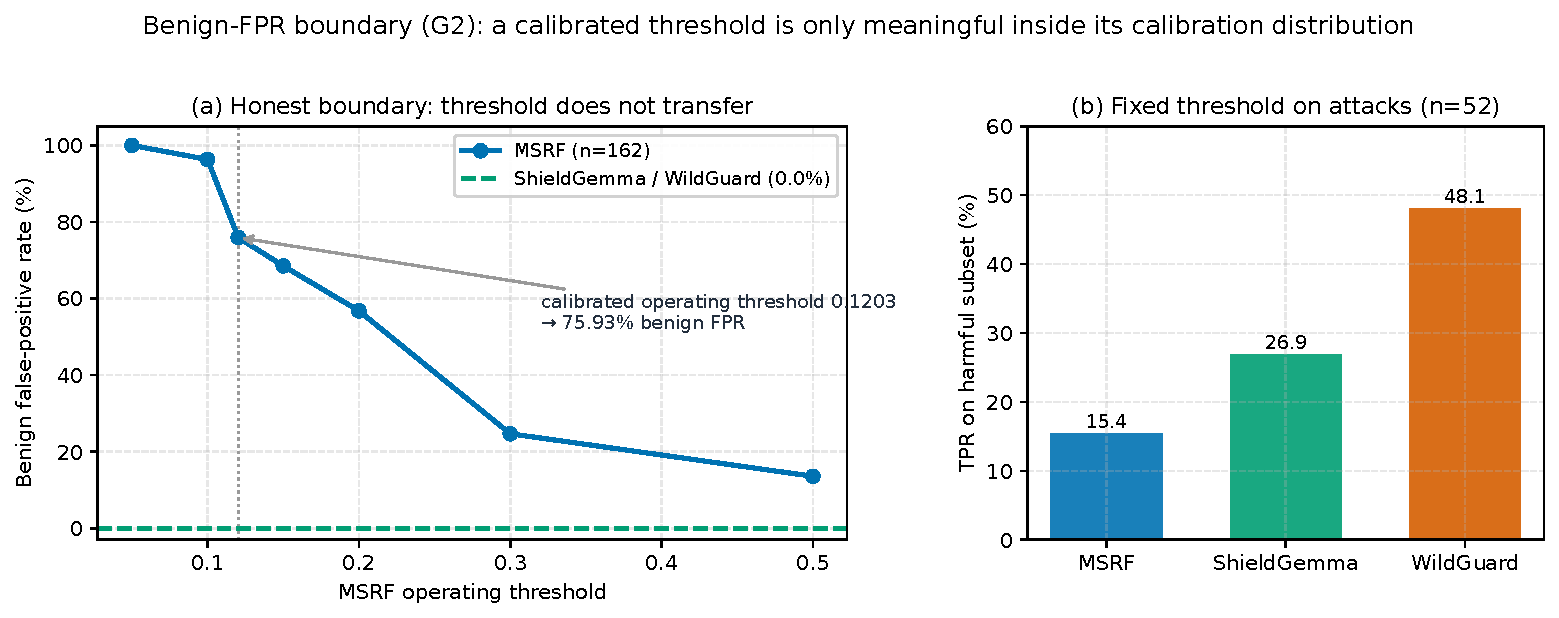
\includegraphics[width=0.88\textwidth]{figures/benign_fpr_boundary.pdf}
\caption{\textbf{Benign-FPR boundary (the G2 criterion).} Rendered as evidence
rather than avoided: (a) \MSRF{} false-positive rate on the independent benign
set ($n=162$) rises to \textbf{75.9\%} at the calibrated operating threshold
0.1203, versus 0.0\% for ShieldGemma and WildGuard; (b) at that \emph{fixed}
threshold, TPR on the harmful subset ($n=52$) is 15.4\% for \MSRF{}, 26.9\% for
ShieldGemma, and 48.1\% for WildGuard --- \MSRF's advantage is in-distribution
discrimination (AUC), not fixed-threshold hit rate on attacks.}
\label{fig:benign-fpr}
\end{figure}

% ======================================================================
% Robustness
% ======================================================================
\subsection{Robustness and adaptive attack}
\label{sec:robustness}

\subsubsection{Defense decay on the attack set}
On a separate attack set ($n=2{,}864$, gray-box and white-box perturbations, each
class $n\geq200$), we re-ran the guards at the response level. On the harmful
subset ($n=52$), \MSRF{} detects 15.4\%, ShieldGemma 26.9\%, WildGuard 48.1\%; on
all rows, \MSRF{} 19.1\%, ShieldGemma 11.3\%, WildGuard 22.2\%. We report these
numbers in full: \MSRF's advantage is in-distribution discrimination (AUC), not
fixed-threshold hit rate on attacks. We also disclose that the attack responses
carry no LoRA intent signal (the intent branch sees an out-of-distribution
zero), which explains part of the decay.

\subsubsection{Adaptive attack decay}
Against the real fused detector, gray-box and white-box perturbation classes
show detection-rate decay up to 20.0~pp relative to baseline. We scope the claim
precisely: our perturbations are single-pass, prompt-level transformations, not
iterative or gradient-based optimization, so we claim \emph{prompt-level
perturbation robustness}, not adversarial robustness in the gradient sense.
Three of six classes are effectively no-ops (fewer than half the perturbations
change the input) and are reported as such rather than as attacks.

\begin{figure}[t]
\centering

\includegraphics[width=0.72\textwidth]{figures/adaptive_decay.pdf}
\caption{\textbf{Detection-rate decay under adaptive perturbations.} The real
fused detector under gray-box and white-box adaptive perturbation classes,
with decay up to 20.0~pp relative to baseline. Perturbations are single-pass,
prompt-level transformations; we claim prompt-level perturbation robustness,
not gradient adversarial robustness.}
\label{fig:adaptive-decay}
\end{figure}

\subsubsection{Audio degradation}
Real audio degradation (Opus 16~kbps, SNR 20~dB, RIR reverberation, each EBU
R128-normalized) changes attack success in opposite directions across models
(e.g., $-7.0$~pp for E2B, $+11.3$~pp for E4B under Opus), which we report as-is.
Degraded audio increases ``thinking-trace leakage'' in one model
(10.0\% / 26.0\% / 28.5\% for the three degradations vs.\ 7.3\% baseline), and
that model's audio-side robustness must not be extrapolated to its text side,
where empty refusals reach 58--85\% (a genuine model behavior we report as such).

\subsubsection{Measurement trust chain}
\label{sec:trust-chain}
We report a five-layer trust chain: deterministic generation (byte-identical,
40/40); scorer reliability (judge\_big vs.\ judge\_small agreement 0.82 on
$n{=}3{,}573$ aligned cells, with Gwet's AC1 0.745 and balanced $\kappa$ 0.706
from the pipeline's agreement utilities \citep{cohen1968}); cross-family
scorer agreement (E4B side 0.929; full E2B text set 0.962); test--retest
agreement (1.000 across three scorers); and Dawid--Skene latent-label recovery
(0.945 in simulation at the measured error regime, 50 replications, 180 items,
$P(\mathrm{harm}){=}0.5$). Batch-inference
byte-equality is not guaranteed (42/200 cells byte-identical, zero errors),
which we disclose in the reproducibility statement.
